\chapter{Introduction: Streaming data science}

As we know, society as a whole is undergoing a data-centered revolution.
The amount of data generated by humans is growing exponentially, and the
need to analyze and extract value from this data is becoming more and more
important. This is especially true in the context of streaming data, where
data is generated continuously and in real-time. \\

The world is characterized by these 4 factors:
\begin{itemize}
    \item \textbf{Volatility}: The speed at which things change.
    \item \textbf{Uncertainty}: The lack of predictability.
    \item \textbf{Complexity}: The number of factors involved.
    \item \textbf{Ambiguity}: The lack of clarity, or the existence of multiple interpretations.
\end{itemize}

In this context, the traditional data science approach is not enough. 
Changes in data can cause the traditional models to become
obsolete, and the need for real-time analysis is becoming more and more
important. This is where streaming data science comes in. In this and the 
following chapters, we will explore the world of streaming data science.\\

Until now, we have assume the data points we receive are independent and 
identically distributed (i.i.d.). But often in real situations,
this assumption doesn't hold:
\begin{itemize}
    \item \textbf{Non identically distributed data}: changes happen, and produce 
    different data distributions for the same data source.
    
    \item \textbf{Non independent data}: data points may not be independent from each
    other. Furthermore, in many cases we have a strong temporal dependency between
    data points.
\end{itemize}

To deal with these situations, we have many approaches, depending on the conditions of
the problem: \textbf{Time Series Analysis}, \textbf{Streaming Machine Learning} and also
\textbf{Continual AI}. 

\begin{figure}[H]
    \centering
    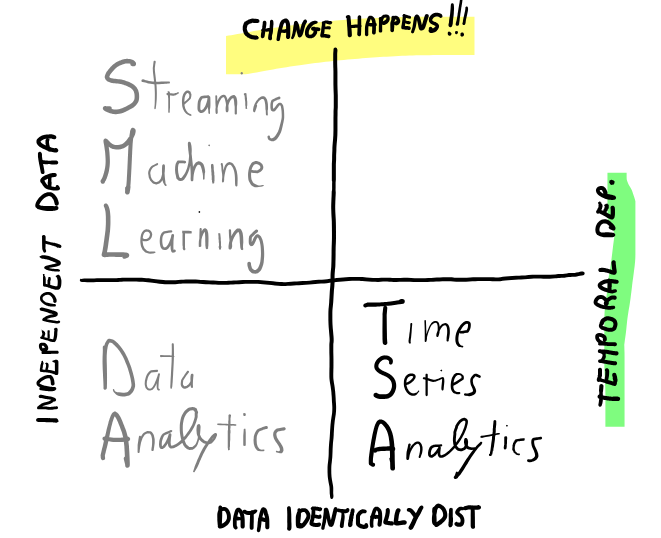
\includegraphics[width=0.5\textwidth]{figures/stream_data_science_approaches.png}
    \caption{Approaches to deal with streaming data science.}
    \label{fig:stream_data_science_approaches}
\end{figure}

\section{Time Series Analysis}

Time series analysis (TSA) is a statistical technique that deals with time-ordered data.
It allows us to explain the past and forecast the future of a continuos flow of data
\textbf{without assuming data independence}.\\

As the name says, this approach is focused on time series data. A time series is a 
sequence of observations on one (or more) quantitative variable \textbf{regularly
collected over time}. In here, we need to make the difference between time series
and events:
\begin{itemize}
    \item In \textbf{events}, the phenomenon happens and it is observed \textbf{irregularly} (the
    observations are note necessarily regularly spaced in time).

    \item In \textbf{time series}, we monitor the phenomenon \textbf{regularly} 
    (the observations are regularly spaced in time).
\end{itemize}

\begin{figure}[H]
    \centering
    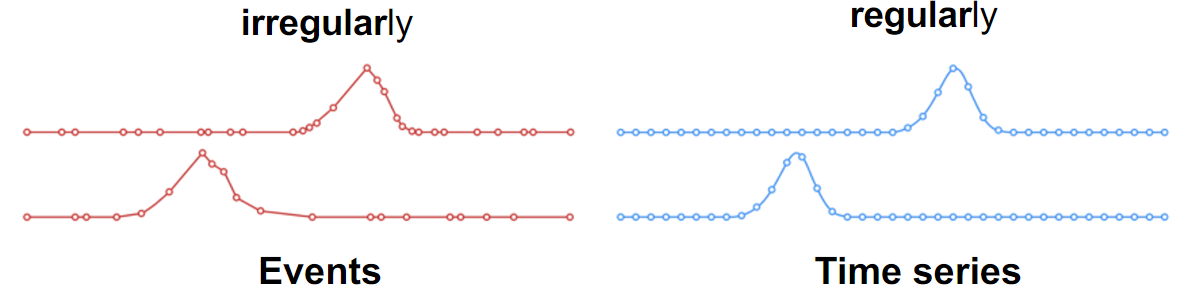
\includegraphics[width=0.8\textwidth]{figures/events_vs_TS.png}
    \caption{Time series vs events}
    \label{fig:time_series_vs_events}
\end{figure}

Note that we can convert events into time series by \textbf{windowing} the data.
For example, the average trade price of Apple stock every 10 minutes over the
course of a day; or the average response time for requests in an application over 1
minute intervals.\\

TSA has two main purposes:
\begin{itemize}
    \item \textbf{Modeling (descriptive analysis)}: We want to understand the underlying
    structure of the data, and how it changes over time. Specially, we want to extract 
    the \textbf{trend} and \textbf{seasonality} of the data.

    \item \textbf{Forecasting (predictive analysis)}: We want to predict the future 
    values of the time series, to make decisions based on this predictions.

\end{itemize}

Note also that TSA is \textbf{not inherently adaptive} nor focused on real-time 
learning. Models are (almost always) retrained from scratch when new data is available.
For this, we need to use \textbf{Streaming Machine Learning}.

\section{Streaming Machine Learning}

Streaming Machine Learning (SML) is a subfield of machine learning that deals with
data that is generated continuously and in real-time. It allows us to learn one data at
a time from a continuous flow of data \textbf{without assuming identically
distributed data}.\\

In SML, the type of data we receive arrives in a continuous stream, potentially in 
real-time, and we assume that data points are \textbf{independent}, but the \textbf{data
distribution can change over time}.\\

The purpose of SML is to \textbf{extract the insights} from the data as it arrives, and
discard the data points once they have been used. Often, we have a \textbf{low-latency}
requirement and a \textbf{minimal computation footprint}. Classification tasks are the main
application domain of SML, but also forecasting and clustering are in scope.\\

Notice that data can arrive in a continuous stream as easy as a \textbf{balanced} one, 
or as complex as a \textbf{dynamically imbalanced} one.\\

\subsection{Techniques in SML: Overview}

Some techniques used in SML are the \textbf{Hoeffding trees}: these are decision trees
\textbf{built incrementally}:

\begin{itemize}
    \item A data point at a time.
    \item Memory stores only the model.
\end{itemize}

For these trees, we have theoretical guarantees that the model will converge to the
tree that would have been built if all the data was available at once.\\

To adapt to the changing data distribution, we can use \textbf{data and concept drift detection}
techniques. These techniques allow us to detect when the data distribution has changed,
and adapt the model accordingly:
\begin{itemize}
    \item We can monitor the input distribution: is there a statictically significant 
    difference between the distribution of the recent data and the distribution of the
    old data? This detects \textbf{data drifts}.

    \item We can monitor the prediction error: is there a statistically significat growth
    between the recent and the old errors? This detects \textbf{concept drifts}.
\end{itemize}

By adding these techniques to the model, we can adapt to the changing data distribution
and keep the model up-to-date. We obtain the \textbf{Hoeffding Adaptive Trees (HAT)}, 
that work as follows:
\begin{itemize}
    \item When a concept drift is detected, start growing alternative branches.
    \item When the alternative branches are better than the current ones, replace them.
\end{itemize}

We also have techniques like \textbf{ensembles}, that combine multiple models to improve
the performance of the model. We have:
\begin{itemize}
    \item \textbf{Bagging}: We train multiple models on different subsets of the data, and
    combine the predictions of these models.
    
    \item \textbf{Boosting}: We train multiple models sequentially, and each model is trained
    to correct the errors of the previous model.
\end{itemize}

\subsection{Learning characteristics and challenges}

SML is \textbf{adaptive} and designed to handle \textbf{changing data distributions} and
\textbf{concept drifts}. Ir is well-suited for applicationts requiring \textbf{immediate 
response} to incoming data changes.\\

However, SML has this immediate reaction to changes at a sometimes high cost: \textbf{it forgets}.
This is, the model is not able to remember the past data, and it can only learn from the
data that is currently available. This can lead to \textbf{catastrophic forgetting}, where
the model forgets the past data and becomes obsolete.

\begin{figure}[H]
    \centering
    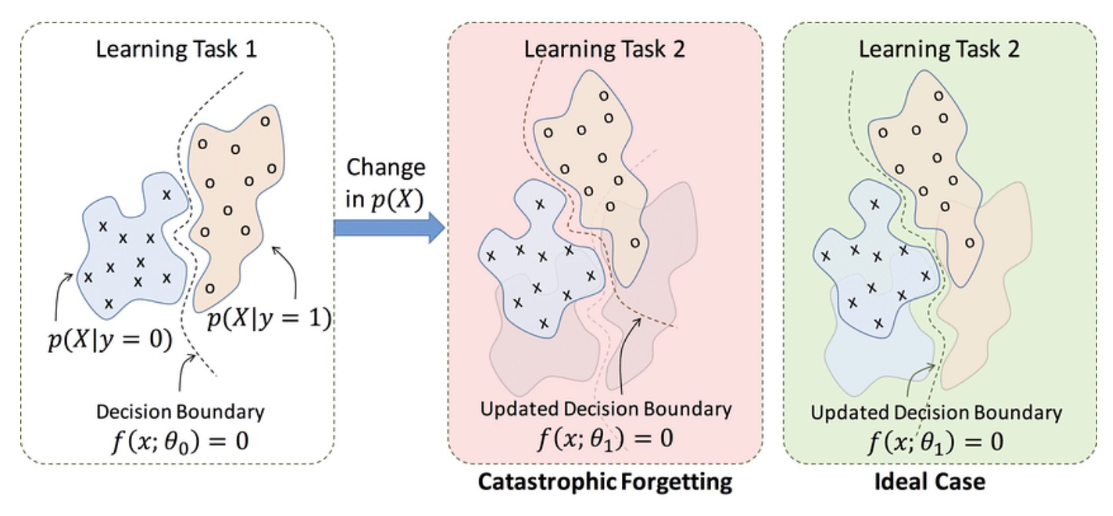
\includegraphics[width=0.8\textwidth]{figures/catastrophic_forgetting.png}
    \caption{Catastrophic forgetting}
    \label{fig:catastrophic_forgetting}
\end{figure}

This illustrates the \textbf{plasticity-stability dilemma} in AI:

\begin{itemize}
    \item \textbf{Plasticity}: The ability of the model to adapt to new data.
    \item \textbf{Stability}: The ability of the model to retain the knowledge of the past data.
\end{itemize}

If a model is too plastic, it will forget the past data and become obsolete. If a model is
too stable, it will not adapt to the new data and will not be able to learn from it.\\

To solve this dilemma, we need to use \textbf{Continual AI}.

\section{Continual AI}

Continual AI (CAI) is a subfield of AI that allows us to build a model that
learns from a sequence of training episodes intermixed with situations that require
applying (recently or prevously) learned skills.\\

In this case, data arrives in (often manually drafted) \textbf{experiences}, where training
and test episodes \textbf{intermix}, assuming that data points are \textbf{independent and
identically distributed only within each experience}. Data in two experiences are normally
distributed differently.\\

As an example, we have the training of a robotic arm to perform various tasks. 
The following diagram shows the key features of CAI.

\begin{figure}[H]
    \centering
    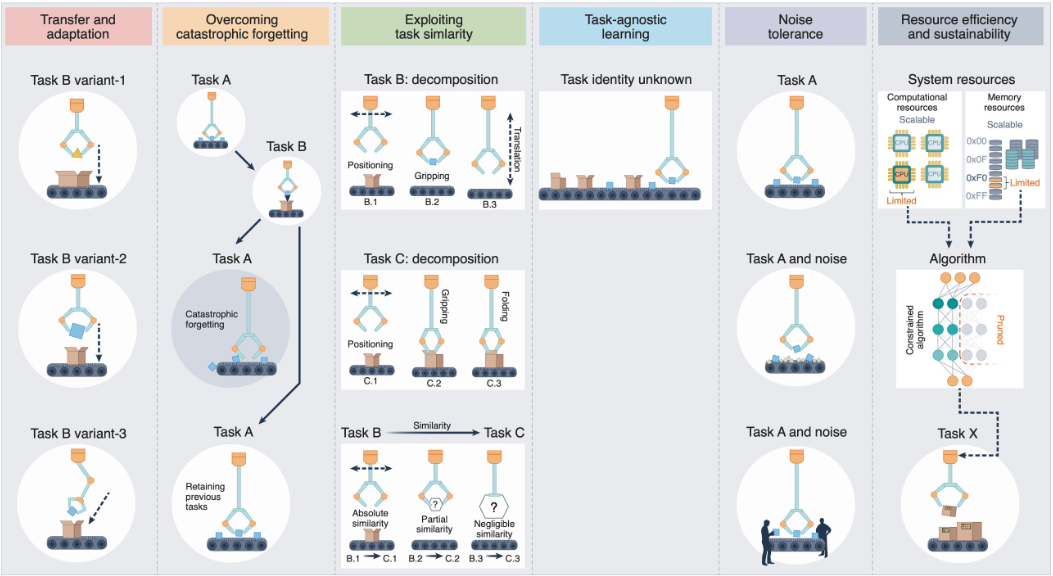
\includegraphics[width=0.8\textwidth]{figures/CAI.png}
    \caption{Continual AI}
    \label{fig:CAI}
\end{figure}

CAI is primarily used to \textbf{avoid catastrophic forgetting} while learning new 
experiences. It balances between \textbf{plasticity} and \textbf{stability}, potentially
via task similarity. Eventually, it also learns when the task identity is unknown, 
tolerates noise and it is more prone to resource constraint environments.

\subsection{Techniques in CAI: Overview}

In CAI, we will take a look at two main techniques:

\begin{itemize}
    \item \textbf{Rehearsal strategies (episodic replay)}: alleviate catastrophic
    forgetting by:
    \begin{itemize}
        \item storing past data points in an episodic memory system.
        \item regularly replaying past data points with real ones from the
        new task.
        \item learning from the obtained mix of replayed and real data points.
    \end{itemize}

    \item \textbf{Architectural strategies (neurogenesis)}: alleviate catastrophic
    forgetting by:
    \begin{itemize}
        \item choosing specific deep learning architectures, layers,
        activation functions, etc.

        \item weight-freezing and dynamic architectures (e.g., adding
        new layers).
    \end{itemize}
\end{itemize}

\subsection{Learning characteristics}

Continual Learning ensures that models can \textbf{adapt to new information} while \textbf{
retaining previously learned knowledge}. It focuses on long-term model stability.

\section{Summary}

In summary, streaming machine learning is designed for real-time
data stream processing and model adaptation, time series analytics is
primarily retrospective and focuses on historical data analysis, while
continual learning is concerned with the long-term adaptation of
models to new data while avoiding forgetting essential knowledge.\\

The choice of approach depends on the specific requirements of the application
and the nature of data being analysed.


